 \documentclass[a4paper,12pt]{article}
%%%%%%%%%%%%%%%%%%%%%%%%%%%%%%%%%%%%%%%%%%%%%%%%%%%%%%%%%%%%%%%%%%%%%%%%%%%%%%%%%%%%%%%%%%%%%%%%%%%%%%%%%%%%%%%%%%%%%%%%%%%%%%%%%%%%%%%%%%%%%%%%%%%%%%%%%%%%%%%%%%%%%%%%%%%%%%%%%%%%%%%%%%%%%%%%%%%%%%%%%%%%%%%%%%%%%%%%%%%%%%%%%%%%%%%%%%%%%%%%%%%%%%%%%%%%
\usepackage{eurosym}
\usepackage{vmargin}
\usepackage{amsmath}
\usepackage{multicol}
\usepackage{graphics}
\usepackage{epsfig}
\usepackage{framed}
\usepackage{subfigure}
\usepackage{fancyhdr}
\usepackage{enumerate}
\setcounter{MaxMatrixCols}{10}
%TCIDATA{OutputFilter=LATEX.DLL}
%TCIDATA{Version=5.00.0.2570}
%TCIDATA{<META NAME="SaveForMode" CONTENT="1">}
%TCIDATA{LastRevised=Wednesday, February 23, 2011 13:24:34}
%TCIDATA{<META NAME="GraphicsSave" CONTENT="32">}
%TCIDATA{Language=American English}

%\pagestyle{fancy}
\setmarginsrb{20mm}{0mm}{20mm}{25mm}{12mm}{11mm}{0mm}{11mm}
%\lhead{MA4413 2013} \rhead{Mr. Kevin O'Brien}
%\chead{Midterm Assessment 1 }
%\input{tcilatex}

\begin{document}
	
	\begin{center}
		
\includegraphics[scale=0.60]{shieldtransparent2}
	\end{center}
	
	\begin{center}
		\vspace{1cm}
		\large \bf {FACULTY OF SCIENCE AND ENGINEERING} \\[0.5cm]
		\normalsize DEPARTMENT OF MATHEMATICS AND STATISTICS \\[1.25cm]
		\large \bf {END OF SEMESTER EXAMINATION} \\[1.5cm]
	\end{center}
	
	\begin{tabular}{ll}
		MODULE CODE: MA4128 & SEMESTER: Spring 2018\\[1cm]
		MODULE TITLE: Advanced Data Modelling & DURATION OF EXAM: 2.5 hours \\[1cm]
		LECTURER: Kevin O'Brien & GRADING SCHEME: 100 marks\\
		& \phantom{GRADING SCHEME:} \footnotesize {60\% of total module marks}   \\[0.8cm]
		EXTERNAL EXAMINER: Prof. A Marshall & \\[1cm]
		\\[1cm]
	\end{tabular}
	\begin{center}
		{\bf INSTRUCTIONS TO CANDIDATES}
	\end{center}
	
	{\noindent \\ This paper is comprised of five questions, each worth 25 marks. Attempt any four questions.
		\\ Scientific calculators approved by the University of Limerick can be used. 
		\\ Statistical tables are provided at back of exam paper.
	}
	\normalsize
	\newpage

%%%%%%%%%%%%%%%%%%%%%%%%%%%%%%%%%%%%%%%%%%%%%%%%%%%%%%%%%%%%
% Dixon Q-Test (4 Marks)
% Grubbs Test (3 Marks)
% ShapiroTest (4 Marks)
% QQplot (3 Marks)
% Missing Data (11 Marks)


\begin{enumerate}
	\item 
	\begin{enumerate}[(a)]
%		\item (4 Marks) Provide a brief description for three tests from the family of Grubb's  Outliers Tests. Include in your description a statement of the null and alternative hypothesis for each test, any required assumptions and the limitations of these tests.			
		\item  (4 Marks) Showing your working, use the Dixon Q Test test that there is no outlier present in the following data set.
		\[ \{112, 167, 140, 129, 125, 139, 117, 135, 131, 119\}\]
	\smallskip
	\item The following statistical procedure is based on this dataset.
\[\{6.98, 8.49, 7.97, 6.64,
			8.80, 8.48, 5.94, 6.94,
			6.89, 7.47, 7.32, 4.01\}
	\]
	
	\begin{framed}
		
		\begin{verbatim}
		> grubbs.test(x, two.sided=T)
		
		Grubbs test for one outlier
		
		data:  x
		G = 2.4093, U = 0.4243, p-value = 0.05069
		alternative hypothesis: lowest value 4.01 is an outlier
		\end{verbatim}
	\end{framed}
	
	\begin{itemize}
		\item[(i)] (2 Marks) Describe the purpose of this procedure. State the null and alternative hypotheses. 
		\item[(ii)] (1 Mark) Write the conclusion that follows from the code output above.
		\item[(iii)] (1 Mark) State any relevant assumptions for this procedure.
	\end{itemize}
\bigskip
\item 
Consider the following inference procedure performed on data set $X$.
\begin{framed}
	\begin{verbatim}
	> shapiro.test(X)
	
	Shapiro-Wilk normality test
	
	data:  X
	W = 0.84987, p-value = 2.143e-13
	
	\end{verbatim}
\end{framed}


\begin{itemize}
	\item[(i)] (2 Marks) Describe the purpose of this procedure. Include in your answer how the outcome of the procedure is to be interpreted.
	\item[(ii)] (3 Marks) What is the null and alternative hypotheses for this test? Write the conclusion that follows from this procedure.
\medskip


\noindent \textit{This question is continued on the next page.}
	
\newpage	
\item[(iii)] (2 Marks) A subsequent procedure is reported below. Describe what was attempted in the procedure, and the outcome. Suggest a possible reason for this outcome.
\end{itemize}

\begin{framed}
\begin{verbatim}
> X <- log(X)
>
> shapiro.test(logX)
	
Shapiro-Wilk normality test
	
data:  X
W = NaN, p-value = NA
\end{verbatim}
\end{framed}



%
%\item A graphical procedure was carried out to assess whether or not this assumption of normality is valid for data set \texttt{Y}. Consider the normal probability plot (i.e. Q-Q plot) in the figure below.
%
%\begin{center}
%	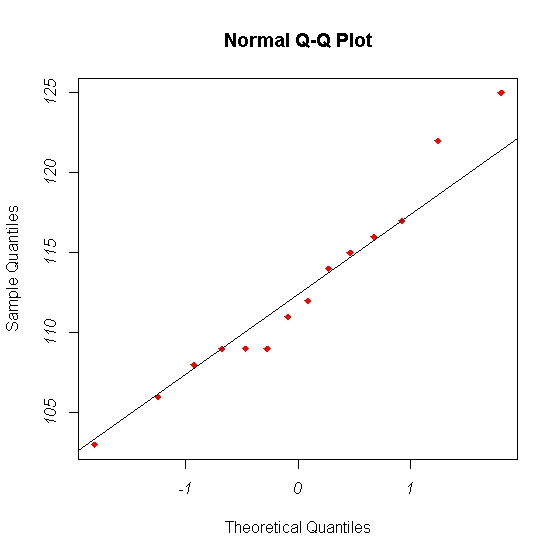
\includegraphics[scale=0.55]{Q5examQQplot}
%\end{center}
%
%\begin{itemize}
%	\item[(i)] (2 Marks) Provide a brief description on how to interpret plots such as this. Support your answer with sketches.
%	\item[(ii)] (1 Mark) What is your conclusion for this procedure? Justify your answer.
%\end{itemize}

%=========================================================%
\bigskip
	\item The following questions relate to Missing Data.
\begin{enumerate}[(i)]
	\item (2 Marks) What is Missing Data? Discuss the implications of Missing Data in the context of a statistical analysis.
	\item (3 Marks) Compare and contrast the following types of missing data: Missing At Random, Missing Not At Random, Missing Completely at Random.
%	\item (3 Marks) Discuss some of the traditional techniques for dealing with Missing Data, making reference to the limitations of each.
	\item (5 Marks) Describe the technique of Multiple Imputation.

%
%	\item (4 Marks) Explain what is meant by Censored Data and Truncated Data. Explain three different types of Censored data.
\end{enumerate}
	
%\item The following questions relate to Numeric Transformation of Data
%		
%		
%		\begin{itemize}
%			\item[(i)] (2 Marks) Describe the purpose of transformations
%		%	\item[(ii)] (2 Marks) Describe the process of transformations
%			\item[(ii)] (2 Marks) Describe the purpose of Tukey's Ladder (referencing direction and relative strength)
%			\item[(iii)] (2 Marks) Give an example of a transformation for various types of skewed data (use Tukey's Ladder, with an example for both directions)
%			\item[(iv)] (2 Marks) Describe the limitations of transformations
%		\end{itemize}


	\end{enumerate}
%%%%%%%%%%%%%%%%%%%%%%%%%%%%%%%%%%%%%%%%%%%%%%%%%%%%%%%%%%%%%%%%%%%%%%%%%%%%%
\newpage
	\item 

% ROC Curve
% Accuracy Precision Recall
% Dummy Variables

 
	\begin{enumerate}[(a)]


	%	\item (3 Marks)	Explain the following terms:  confusion matrix,  prior probabilities cost of misclassification, and apparent error rate.

		\item (3 Marks) With reference to the table below, define each of the following appraisal metrics in the context of a binary classification procedure (\textit{1 Mark for each}).
		\begin{enumerate}[(i)]
			\item Accuracy
			\item Precision
			\item Recall
		\end{enumerate}
		\begin{center}
		\begin{tabular}{|c|c|c|}
			\hline  & Predicted Negative & Predicted Positive \\ 
			\hline Observed Negative & True Negative & False Positive \\ 
			\hline Observed Positive & False Negative & True Positive \\ 
			\hline 
		\end{tabular} 
	\end{center}
\bigskip
		\item (2 Marks) What is the F-score? Explain why the F-score is considered a more informative measure of performance than the Accuracy score.
		
		\[ \mbox{Hint:    }\;\;\;\; \mbox{F-score} = \frac{2\times P \times R}{P + R} \]
%		\item (2 Marks) Define Specificity and Sensitivity. You make reference to previous answers.
		
\bigskip		
\item (3 Marks) Calculate the following appraisal metrics using the below table of outcomes for binary classification \textit{(1 Mark for each)}.
\begin{itemize}	
	%	\item[(i)] (1 Mark)	Accuracy,
		\item[(i)] 	Recall,
		\item[(ii)] Precision,
		\item[(iii)] F-score.
\smallskip
\begin{center}
	\begin{tabular}{|c|c|c|}
		\hline  & \phantom{spa}Predict Negative\phantom{spa} & \phantom{spa}Predict Positive\phantom{spa} \\ 
		\hline\phantom{spa} Observed Negative \phantom{spa}&	9710	&	90	\\ 
		\hline \phantom{spa}Observed Positive\phantom{spa} & 	80	&	120	\\ 
		\hline 
	\end{tabular} 
\end{center}	
		\end{itemize}
	
			%	\item[(iii.)](2 Marks) Define Specificity and Sensitivity. You make reference to previous answers.
			
\bigskip
		\item (3 Marks) What is a Receiver Operator Character (ROC) curve? Explain its function in the context of a binary classification procedure, how it is determined, and the means of interpreting the curve. Support your answer with sketches.	
	
%	\item (1 Mark)	The apparent error rate calculated when all observations are used to construct the discriminant rules is known to underestimate the true error rate.  What can be done to overcome this problem?
%	\item  Briefly describe what a variable selection procedure is?
\bigskip 


\item Answer the following questions relating to the SPSS output on the next page. In this analysis, we wish to predict whether or not a person has a saving's account, based on the following demographic variables.

\begin{itemize}
	\item Age
	\item Socio-economic Status
	\item Sector within city
	\item Disease Status
\end{itemize}
There are three possible outcomes for socio-economic status.
\[\{\mbox{1 = Upper, 2 = Middle, 3 = Lower}\}\]

There are three possible outcomes for socio-economic status.
\[\{\mbox{1 = Inner City, 2 = Inner Suburbs, 3 = Outer Suburbs}\}\]

The Disease status variable is a binary variable, with 1 indicating the presence of some sort of illness.

\noindent \textit{This question is continued on the next page.}





\begin{enumerate}[(i)]
\item (1 Mark) Describe how Wald's Test was used to refine the initial model. Make reference to relevant figures in the output.
\item (2 Marks)
What is a logit? How can you transform a logit into a probability?

\item (1 Mark) State the regression equation for the final logistic regression model.
\item (4 Marks) What information is contained in the column labeled \texttt{Exp(B)}? For the initial model, interpret the figures from this column for both \textbf{\textit{Socioeconomic status}} and \textbf{\textit{Sector within city}}. 
As part of your answer, comment on the 95\% confidence intervals for both.


\item (2 Marks) Predict the outcome for the following case: a 55 year old person from the upper socio-economic category residing in the outer suburbs.
\item (2 Marks) Predict the outcome for the following case: a 25 year old person  from the middle socio-economic category residing in the inner suburbs.

\item (2 Marks)
What is a dummy variable? Explain how it is used in Logistic Regression. Support your answer with an example.
\end{enumerate}

\begin{figure}[h!]
	\centering

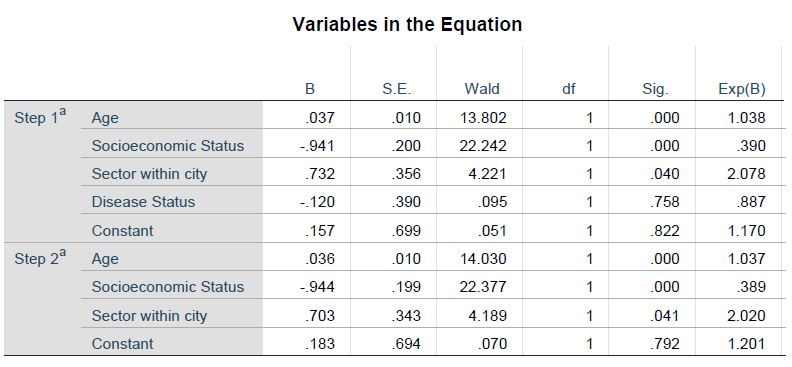
\includegraphics[width=1.00\linewidth]{BLR-A}\\

\end{figure}

\noindent \textit{This question is continued on the next page.}
\begin{figure}[h!]
	\centering

	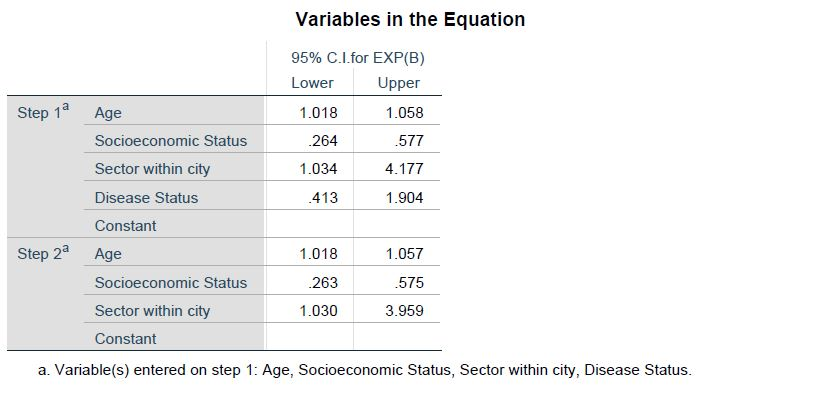
\includegraphics[width=1.00\linewidth]{BLR-B}\\
	
\end{figure}
\end{enumerate}
\newpage
%%%%%%%%%%%%%%%%%%%%%%%%%%%%%%%%%%%%%%%%%%%%%%


	\item 
	\begin{enumerate}[(a)]
%\item (2 Marks)  What is a vertical icicle plot used for? Give a brief description, supporting your answer with sketches.
		\item (4 Marks)  Compute the following distance metrics between the cases A, and B, described below. (\textit{1 Mark for each}).
		\begin{enumerate}[(i)]
		\item Euclidean Distance
		\item Squared Euclidean Distance
		\item Manhattan Distance
		\item Chebyshev Distance
		
	
		\[ A = \{5,9,2,11,4\}\]
		\[ B = \{3,6,9,4,7\}\]
		\item (1 Mark) Explain why the squared Euclidean distance may be used in preferences in to the Euclidean Distance.
	\end{enumerate}
%		\item Cosine Similarity. Support your answer with a sketch.
%		\item Mahalanobis Distance. Support your answer with a sketch.



\bigskip 
\item The following questions relate to Hierarchical Clustering.


\begin{enumerate}[(i)]
\item (1 Mark) Distinguish between agglomerative and divisive hierarchical clustering techniques.
	
\item (3 Marks) Why do you standardize variables before carrying out a cluster analysis. Support your answer with an example.

\item (3 Marks) Describe the process of Ward's Linkage in the context of cluster analysis.


\noindent \textit{This question is continued on the next page.}
\newpage	
\item (9 Marks)  Describe any three of the following linkage methods. Support your answer with sketches (\textit{3 Marks for each}).
	\begin{itemize}
		\item Nearest Neighbour Linkage
		\item Furthest Neighbour Linkage
		\item Centroid Linkage
		\item Average Linkage
	\end{itemize}

	\item (2 Marks) In the context of cluster analysis, What is the chaining effect? Give a brief description, supporting your answer with sketches.
%	
	\item (2 Marks) Describe how a dendrogram would assist in the interpretation of a hierarchical clustering solution. Support your answer with a sketch.
	

	
\end{enumerate}


	
	\end{enumerate}

%%%%%%%%%%%%%%%%%%%%%%%%%%%%%%%%%%%%%%%%%%%%%%%%%%%%%%%%%%%%%%%%%%%%%%%%%%%%%%%%%
\newpage

	\item 
	\begin{enumerate}[(a)]

%%%%%%%%%%%%%%%%%%%%%%%%%%%%%%%%%%%%%%%%%%%5

\item The following questions relate to K-means Clustering.

\begin{enumerate}[(i)]
	\item (1 Mark) Compare and contrast k-means clustering and hierarchical clustering in terms of the number of clusters determined.
	\item (7 Marks) Explain the process of k-means clustering, starting with an initial cluster allocation. 
	You may work on the basis of a two-cluster solution. Support your answer with several sketches.
	\item(2 Marks) Describe a graphical procedure to assist in determining the appropriate number of clusters.
	
	\item (2 Marks) For a 4 cluster k-means solution, interpret the ANOVA table below.
\end{enumerate}


\begin{figure}[h!]
	\centering
	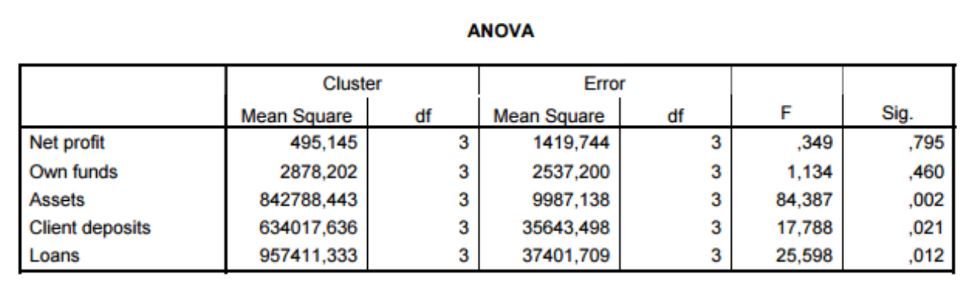
\includegraphics[width=0.9\linewidth]{Cluster}
\end{figure}


% \item (1 Mark) What is the theoretical difference between principal components analysis and factor analysis?
	 
%	\end{enumerate}
%
%
%
%%\subsection*{Question 3 :k-means cluster analysis}
%%Use two clusters.
%%Illustrate your answer with sketches.
%
%\newpage
%
%\item 
%\begin{enumerate}[(a)]
\item The following topics relate to techniques for predictive modeling count techniques.


\begin{itemize}
	\item[(i)] (2 Marks)
	What does a Poisson regression model? State any assumptions that must be checked before it can be used.
	%	Poisson Processes and Count Variables
	%	Be able to give some examples
	%	Checking 
	%
	%	Simulation Studies to Check range of ratio values to be expected.
	
	\item[(ii)] (1 Mark) The \texttt{R} Code output given below is used to predict the number of awards won by students. \begin{itemize} 
		\item[$\bullet$] Information is provided on which of the three school programs the student takes part in (\textit{General}, \textit{Vocational} or \textit{Academic}). 
		\item[$\bullet$] Also we are given the mathematics test score.
	\end{itemize}
	State the mathematical formula used to predict the number of awards won.\\
	\textit{You can denote \textbf{progAcademic}, \textbf{progVocational} and \textbf{math} as $x_1$,$x_2$ and $x_3$ respectively.}
	
	
	\begin{framed}
		\begin{verbatim}
		Coefficients:
		               Estimate Std. Error z value Pr(>|z|)    
		(Intercept)     -5.2471     0.6585   -7.97  1.6e-15 ***
		progAcademic     1.0839     0.3583    3.03   0.0025 ** 
		progVocational   0.3698     0.4411    0.84   0.4018    
		math             0.0702     0.0106    6.62  3.6e-11 ***
		---
		Signif. codes:  0 '***' 0.001 '**' 0.01 '*' 0.05 '.' 0.1 ' ' 1
		
		\end{verbatim}
	\end{framed}

\noindent \textit{This question is continued on the next page.}
\newpage
	\item[(iii)] (2 Marks) Use the model in Part (ii) to predict the number of awards won by a general program student, with a maths score of 55.
	
	\item[(iv)] (2 Marks) Use the model in Part (ii) to predict the number of awards won by an academic program student, with a maths score of 75.
	
	\item[(v)] (1 Mark) Describe the circumstances whereby Negative Binomial Regression Models would be used instead of Poisson Models.	
	\item[(vi)] (3 Marks)
	What is Zero Inflation? Explain the modeling process for a Zero Inflated Model. Give an example of Zero-Inflated Count Process. \textit{Support your answer with a sketch, if necessary.}
	
	

	
	
	
	\item[(vii)] (2 Marks) What is Zero Truncation? Give an example of a Zero Truncated Count Process.
\end{itemize}


\end{enumerate}
\bigskip
%%%%%%%%%%%%%%%%%%%%%%%%%%%%%%%%%%%%%%%%%%%%%%%%%%%%%%%%%%%%%%%%%%%%%%%%%%%%%
\item 
\begin{enumerate}

	\item The following questions relate to multicollinearity in the context of multiple
regression analysis.
\begin{enumerate}[(i)]
	\item (1 Mark) Define multicollinearity.
	\item (2 Marks) State two ways in which a multiple regression analysis could be affected by severe
	multicollinearity.
	\item (2 Marks) State two ways of formally diagnosing the severity of multicollinearity, making reference to how both should be used to make decisions about the data.
	%	\item  Describe two statistical methods that can be applied to the data to lessen the effects of severe multicollinearity.
\end{enumerate}

%\item Write a brief explanation of how robust regression differs from linear models computed using
%the Ordinary Least Squares method, making reference to one particular weighting method.
\bigskip
\item 
The following questions relate to Principal Component Analysis.
\begin{enumerate}[(i)]
	
	\item (2 Marks)	What is the purpose of a principal component analysis?
	\item (1 Marks) Principal Component Analysis is a Dimensionality Reduction technique. Explain what this term means.
	\item (4 Marks)	What is meant by the ``true" dimension of the data?  How does an analyst determine the appropriate number of principal components to retain, making reference to three different approaches.
	%	\item (2 Marks)	What problems occur if a principal component analysis is carried out on a data matrix where the columns contain measurements on very difference scales?  What can be done to overcome this problem?
	\item (3 Marks) The Kaiser-Meyer-Olkin (KMO) statistic is used to measure a certain characteristic of the data. What is this characteristic? Explain how the KMO statistic should be interpreted.
	\item (2 Marks) Briefly describe the Bartlett Test for Sphericity, with reference to the null and alternative hypotheses, and how those statements relate to the purpose of the test.
\end{enumerate}

\bigskip



\item The following questions relate to model selection and validation in the context of multiple
regression analysis.
\begin{enumerate}[(i)]

	\item (1 Mark) Explain the purpose of variable selection procedures.
	
	\noindent \textit{This question is continued on the next page.}
\newpage
\item (3 Marks) Compare and contrast the following variable selection procedures (\textit{1 Mark for each}).
\begin{itemize}

		\item Forward Selection
		\item Backward Elimination
		\item Stepwise Regression
	\end{itemize}


	\item (1 Mark)  Explain how the \emph{Akaike information criterion} is used to compare two models fitted for the same data.

\item (1 Mark) Explain why the adjusted $R^2$ value may differ in value from the corresponding multiple $R^2$ value for the same fitted model.

	\item (3 Marks) Describe model validation in the model-building process, with particular emphasis on the standard data partition.
\end{enumerate}
\item (5 Marks) For the computer code output on the following pages, there are 7 iterations of a model fitting process. The response variable is denoted $Y$, and the predictor variables are denoted $V1$ to $V10$. Describe what the process is doing, stating how and what conclusion is reached. 
\end{enumerate}


\end{enumerate}


\noindent \textbf{Iteration 1}
\begin{framed}
	\begin{verbatim}
	Start:  AIC = -1107.36
	Y ~ V1 + V2 + V3 + V4 + V5 + V6 + V7 + V8 + V9 + V10
	
	       Df Sum of Sq     RSS      AIC
	- V5    1   0.00005 0.91210 -1109.35
	- V4    1   0.00012 0.91217 -1109.33
	- V2    1   0.00241 0.91446 -1108.81
	- V7    1   0.00517 0.91722 -1108.18
	- V3    1   0.00576 0.91781 -1108.05
	- V1    1   0.00784 0.91989 -1107.58
	<none>              0.91205 -1107.36
	- V8    1   0.00972 0.92177 -1107.15
	- V6    1   0.01340 0.92544 -1106.32
	- V9    1   0.02434 0.93639 -1103.88
	- V10   1   0.72914 1.64118  -987.16
	\end{verbatim}
\end{framed}
\newpage
\noindent \textbf{Iteration 2}
\begin{framed}
	\begin{verbatim}
	Step:  AIC = -1109.35
	Y ~ V1 + V2 + V3 + V4 + V6 + V7 + V8 + V9 + V10
	
	Df Sum of Sq     RSS      AIC
	- V4    1   0.00038 0.91248 -1111.26
	- V2    1   0.00238 0.91448 -1110.80
	- V7    1   0.00512 0.91722 -1110.18
	- V3    1   0.00594 0.91804 -1110.00
	- V1    1   0.00779 0.91989 -1109.58
	<none>              0.91210 -1109.35
	- V8    1   0.01000 0.92210 -1109.08
	- V6    1   0.01761 0.92971 -1107.37
	+ V5    1   0.00005 0.91205 -1107.36
	- V9    1   0.02431 0.93641 -1105.87
	- V10   1   0.72945 1.64155  -989.11
	\end{verbatim}
\end{framed}

\noindent \textbf{Iteration 3}
\begin{framed}
	\begin{verbatim}
	Step:  AIC = -1111.26
	Y ~ V1 + V2 + V3 + V6 + V7 + V8 + V9 + V10
	
	Df Sum of Sq     RSS      AIC
	- V2    1   0.00224 0.91472 -1112.75
	- V7    1   0.00534 0.91782 -1112.04
	- V3    1   0.00679 0.91927 -1111.72
	- V1    1   0.00753 0.92001 -1111.55
	<none>              0.91248 -1111.26
	- V8    1   0.01006 0.92254 -1110.98
	+ V4    1   0.00038 0.91210 -1109.35
	- V6    1   0.01739 0.92987 -1109.33
	+ V5    1   0.00031 0.91217 -1109.33
	- V9    1   0.02411 0.93659 -1107.83
	- V10   1   0.73044 1.64292  -990.94
	\end{verbatim}
\end{framed}
\newpage
\noindent \textbf{Iteration 4}
\begin{framed}
	\begin{verbatim}
	Step:  AIC = -1112.75
	Y ~ V1 + V3 + V6 + V7 + V8 + V9 + V10
	
	Df Sum of Sq     RSS      AIC
	- V3    1   0.00459 0.91930 -1113.71
	- V1    1   0.00529 0.92001 -1113.55
	- V7    1   0.00578 0.92050 -1113.44
	<none>              0.91472 -1112.75
	- V8    1   0.00970 0.92442 -1112.55
	+ V2    1   0.00224 0.91248 -1111.26
	- V6    1   0.01737 0.93209 -1110.84
	+ V4    1   0.00023 0.91448 -1110.80
	+ V5    1   0.00017 0.91455 -1110.79
	- V9    1   0.02429 0.93900 -1109.30
	- V10   1   0.73427 1.64898  -992.17
	\end{verbatim}
\end{framed}

\noindent \textbf{Iteration 5}
\begin{framed}
	\begin{verbatim}
	Step:  AIC = -1113.71
	Y ~ V1 + V6 + V7 + V8 + V9 + V10
	
	Df Sum of Sq     RSS      AIC
	- V7    1   0.00772 0.92703 -1113.97
	<none>              0.91930 -1113.71
	- V8    1   0.00938 0.92869 -1113.60
	+ V3    1   0.00459 0.91472 -1112.75
	- V1    1   0.01641 0.93571 -1112.03
	+ V4    1   0.00120 0.91810 -1111.98
	+ V5    1   0.00016 0.91914 -1111.74
	+ V2    1   0.00003 0.91927 -1111.72
	- V9    1   0.02333 0.94263 -1110.50
	- V6    1   0.02597 0.94527 -1109.91
	- V10   1   0.73279 1.65209  -993.78
	\end{verbatim}
\end{framed}
\newpage
\noindent \textbf{Iteration 6}
\begin{framed}
	\begin{verbatim}
	Step:  AIC = -1113.97
	Y ~ V1 + V6 + V8 + V9 + V10
	
	Df Sum of Sq     RSS      AIC
	- V8    1   0.00403 0.93106 -1115.07
	<none>              0.92703 -1113.97
	+ V7    1   0.00772 0.91930 -1113.71
	+ V3    1   0.00653 0.92050 -1113.44
	+ V4    1   0.00159 0.92544 -1112.33
	- V1    1   0.01678 0.94381 -1112.24
	+ V5    1   0.00047 0.92656 -1112.07
	+ V2    1   0.00011 0.92692 -1111.99
	- V6    1   0.01831 0.94534 -1111.90
	- V9    1   0.02020 0.94723 -1111.48
	- V10   1   0.72507 1.65210  -995.78
	\end{verbatim}
\end{framed}

\noindent \textbf{Iteration 7}
\begin{framed}
	\begin{verbatim}
	Step:  AIC = -1115.07
	Y ~ V1 + V6 + V9 + V10
	
	Df Sum of Sq     RSS      AIC
	<none>              0.93106 -1115.07
	+ V3    1   0.00539 0.92568 -1114.27
	+ V8    1   0.00403 0.92703 -1113.97
	+ V7    1   0.00238 0.92869 -1113.60
	- V9    1   0.01644 0.94750 -1113.42
	+ V4    1   0.00128 0.92978 -1113.35
	+ V5    1   0.00012 0.93095 -1113.09
	+ V2    1   0.00009 0.93097 -1113.09
	- V1    1   0.01857 0.94963 -1112.96
	- V6    1   0.02851 0.95958 -1110.79
	- V10   1   0.72205 1.65311  -997.65
	
	\end{verbatim}
\end{framed}
\newpage
\begin{framed}
	\begin{verbatim}
	Call:
	lm(formula = Y ~ V1 + V6 + V9 + V10, data = Sonar2)
	
	Coefficients:
	(Intercept)           V1           V6           V9          V10  
	0.03883      0.44476      0.21224     -0.16043      0.91507  
	\end{verbatim}
\end{framed}
%%------------------------------------------------------------------ %

%\subsection*{Question 3a : Discriminant Analysis} % 12 Marks
%% Compare and contrast MANOVA

%\begin{itemize}
%\item[i.](2 Marks) What is the purpose of a discriminant analysis?
%\item[ii.](3 Marks) How does discriminant analysis differ from MANOVA?
%\item[iii.](3 Marks)	Discuss the condition that determines whether or not a linear or quadratic discriminant rule should be used in a discriminant analysis.
%%\end{itemize}
%%%---------------------------------------------------------------------%
%%
%%\subsection*{Question 3b : Model Validation} %7 Marks
%%%----GOOD SHAPE
%%\begin{itemize}
%
%
%
%\end{itemize}

%http://www.education.umd.edu/EDMS/student/Exams/PrelimCompSpr09.pdf

%
%%-----------------------------------------------------------%Q4b Ready
%\subsection*{Question 4b : Logistic Regression} %10 Marks
%\begin{itemize}
%\item[i.](3 Marks) Under what circumstances would you use Logistic Regression?
%\end{itemize}
%\newpage


\section*{Tables}
\subsection*{Critical Values for Dixon Q Test}
{
	\Large
	\begin{center}
		\begin{tabular}{|c|c|c|c|}
			\hline  N  & $\alpha=0.10$  & $\alpha=0.05$  & $\alpha=0.01$  \\ \hline
			3  & 0.941 & 0.97  & 0.994 \\ \hline
			4  & 0.765 & 0.829 & 0.926 \\ \hline
			5  & 0.642 & 0.71  & 0.821 \\ \hline
			6  & 0.56  & 0.625 & 0.74  \\ \hline
			7  & 0.507 & 0.568 & 0.68  \\ \hline
			8  & 0.468 & 0.526 & 0.634 \\ \hline
			9  & 0.437 & 0.493 & 0.598 \\ \hline
			10 & 0.412 & 0.466 & 0.568 \\ \hline
			11 & 0.392 & 0.444 & 0.542 \\ \hline
			12 & 0.376 & 0.426 & 0.522 \\ \hline
			13 & 0.361 & 0.41  & 0.503 \\ \hline
			14 & 0.349 & 0.396 & 0.488 \\ \hline
			15 & 0.338 & 0.384 & 0.475 \\ \hline
			16 & 0.329 & 0.374 & 0.463 \\ \hline
		\end{tabular} 
	\end{center}
}

\end{document} 